% Chinese mathematical companion to the English recovery-initialization research draft.
\documentclass[11pt,a4paper]{ctexart}
\usepackage[margin=2cm]{geometry}
\usepackage{amsmath,amssymb,amsthm,booktabs,graphicx,tabularx}
\usepackage[colorlinks=true,urlcolor=blue,linkcolor=blue]{hyperref}
\setlength{\parskip}{4pt}
\newcommand{\R}{\mathbb R}
\newcommand{\sk}[1]{[#1]_\times}
\newcommand{\Proj}{\mathsf P}
\title{测距--惯性初始化：航向候选、多项式干扰与适用边界}
\author{中文数学说明}
\date{2026年11月11日}
\begin{document}
\maketitle
\begin{abstract}
以单标签、已知锚点、异步TWR和IMU为对象，本文集中讨论两项内容：
利用惯性形状和线性干扰消元产生低成本航向候选，以及多项式干扰吸收偏置时保留或消除航向信息的条件。
给出无噪声恢复充分条件、不变性与不可辨识反例，并区分精确投影和数值截断。
400个配对合成窗口比较局部、解析候选、均匀双/四/十二航向起点，报告实际函数评估和串行耗时；
66个真实时间窗口形成的528个相关配置按日志补报终点位置误差。
在30 m距离、3 m锚点高度跨度下，解析候选保持双起点的目标质量，串行桌面计时子集的中位耗时减少约29.4\%。
真实窗口目标miss由87降至40，终点位置收益随日志变化。方法与分析共同给出初始化候选及模型阶数的选择依据。
\end{abstract}

\section{与原文的关系}
Oursland与Mehrabian的RO-MAN 2024论文采用含杆臂的TDoA观测，重点处理大初始航向误差。
其几何输出与本轮观测分别为
\begin{align}
 h_{BA}(X)&=\|p+R\ell-a_B\|-\|p+R\ell-a_A\|,\\
 z_i&=\|p(t_i)-a_i\|+\beta_i+n_i .\label{eq:twr}
\end{align}
本文将捕获阶段具体化为零杆臂TWR窗口初始化，并继续使用$X\in SE_2(3)$与六维IMU偏置的不变跟踪器。
设物理误差为$[\delta\theta_b,\delta v,\delta p,\delta b_g,\delta b_a]$，对应不变坐标满足
\begin{equation}
 \xi_\theta=R\delta\theta_b,\quad
 \xi_v=\delta v+\sk{v}R\delta\theta_b,\quad
 \xi_p=\delta p+\sk{p}R\delta\theta_b.
\end{equation}
因此$P_r=C(X)P_eC(X)^\top$；新位置或速度交接后必须在新状态处重算$C(X)$。
图\ref{fig:overview}概括了本文的初始化流程及航向信息的几何含义。

\begin{figure}[htbp]
 \centering
 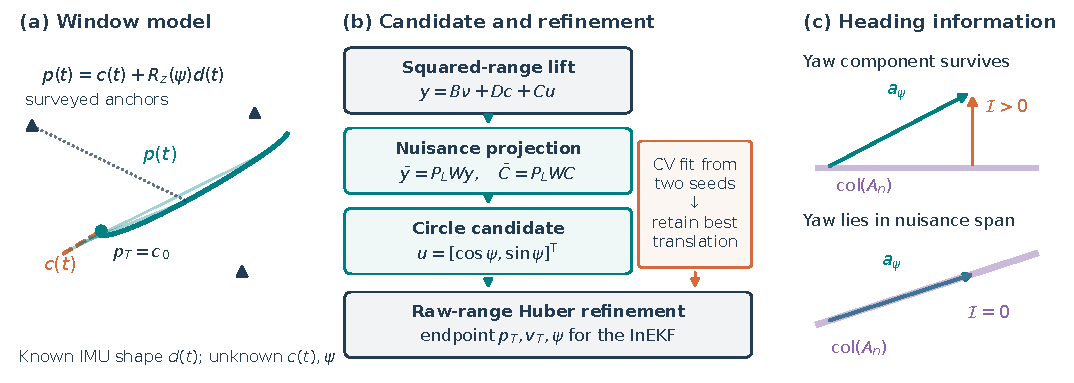
\includegraphics[width=\textwidth]{recovery_bootstrap_figures/method_overview.pdf}
 \caption{方法示意：惯性形状与多项式平移构成窗口轨迹；消元后求圆上的航向候选，与共同CV平移初值配对精化；
 航向信息对应其敏感度在干扰列空间之外的分量。轨迹与投影均为模型示意。}
 \label{fig:overview}
\end{figure}

\section{异步距离中的多项式干扰与航向}
\subsection{窗口模型及平方距离展开}
令$\tau_i=t_i-t_e\leq0$，已知IMU预积分位移为$d_i$，考虑
\begin{equation}
 p_i=\sum_{j=0}^{K}c_j\tau_i^j+R_z(\psi)d_i,\qquad
 u=\begin{bmatrix}\cos\psi&\sin\psi\end{bmatrix}^{\top}.
 \label{eq:model}
\end{equation}
$K=1$对应已校准偏置的惯性窗口；实际回放对$d$作终点重锚，使$d(0)=\dot d(0)=0$，
故$c_0,c_1$分别为终点位置与速度。$K=2$额外吸收常值世界系加速度误差；
只有姿态恒定时，它才与常值机体系加速度偏置严格对应。

定义$r_i=z_i-\beta_i$。忽略噪声时，令
\begin{equation}
 y_i=\tfrac12(r_i^2-\|a_i\|^2-\|d_i\|^2)+a_{iz}d_{iz},
\end{equation}
展开式\eqref{eq:model}得到
\begin{equation}
 y=B\nu+Dc+Cu,
 \label{eq:lift}
\end{equation}
其中
\begin{align}
 B_i&=\big[1,\tau_i,\ldots,\tau_i^{2K},
       (\tau_i^jd_{ix},\tau_i^jd_{iy})_{j=0}^{K}\big],\\
 D_{ij}&=\tau_i^j\big[-a_{ix},-a_{iy},d_{iz}-a_{iz}\big],\\
 C_i&=\big[-a_{ix}d_{ix}-a_{iy}d_{iy},\quad
                 a_{ix}d_{iy}-a_{iy}d_{ix}\big].
\end{align}
$\nu$含$4K+3$个辅助量；$c$含$3K+3$个物理平移系数。
式\eqref{eq:lift}将原本相互约束的辅助量独立化，得到平方距离的\textbf{放松问题}。
在Pacholska等人\emph{Relax and Recover}（RA-L 2020）的测距提升基础上，
本文进一步利用已知惯性形状与单位圆航向结构，把候选生成化为低维问题。

若$n_i\sim\mathcal N(0,\sigma_i^2)$，应从$y_i$中扣除$\sigma_i^2/2$。
在锚点、标定偏置和$d_i$视为确定的条件下，
\begin{equation}
 \operatorname{Var}(y_i)=\rho_i^2\sigma_i^2+\tfrac12\sigma_i^4,
 \qquad \rho_i=\|p_i-a_i\|.
\end{equation}
实际白化权重为$W_{ii}=[\max(r_i,\sigma_i)^2\sigma_i^2+\sigma_i^4/2]^{-1/2}$；
该插件权重近似平方距离方差，后续用原始距离的Huber代价进行鲁棒精化。

\subsection{投影、四次多项式与恢复条件}
记$W$为对角白化权重，$L=W[B\ D]$，
\begin{equation}
 \Proj_L=I-LL^\dagger,\quad \bar y=\Proj_LWy,\quad\bar C=\Proj_LWC.
\end{equation}
理论使用精确列空间投影；实现SVD保留$s_j>10^{-10}s_{\max}$，以低秩分解应用投影而无需形成稠密矩阵。
消元后仅剩二维圆约束问题
\begin{equation}
 \min_{\|u\|=1}\|\bar y-\bar C u\|^2
 =\min_\psi u^\top H u-2g^\top u+\mathrm{const},\quad
 H=\bar C^\top\bar C,\ g=\bar C^\top\bar y.
\end{equation}
令$\Delta=H_{22}-H_{11}$、$s=\tan(\psi/2)$，驻点满足
\begin{align}
0={}&(H_{12}+g_2)s^4+(-2\Delta+2g_1)s^3-6H_{12}s^2\nonumber\\
 &+(2\Delta+2g_1)s+(H_{12}-g_2).
\end{align}
精确枚举实根并补入$\psi=\pi$即可取得该圆问题的全局最小值。
实现将系数按最大幅值归一，绝对值不大于$10^{-13}$的相对系数置零；
接受$|\operatorname{Im}s|<10^{-7}(1+|\operatorname{Re}s|)$的根，额外保留$0,\pi$并按圆代价排序。
多候选按$10^{-7}$ rad去重；常数圆代价保留辅助角度，再交给原始距离精化。

\textbf{恢复条件。}若模型准确、无噪声且$\operatorname{rank}(\bar C)=2$，真实航向是放松圆问题唯一全局最优。
证明：真实解成本为零，其他全局最优必满足$\bar C(u-u_*)=0$，满列秩推出$u=u_*$。
若另外$\operatorname{rank}(\Proj_{WB}WD)=3(K+1)$，平移系数亦唯一。
这些充分条件刻画放松候选模块的可恢复性。实际流程取提升得到的航向，
配合鲁棒常速度平移初值优化原始距离。

\subsection{多项式污染不变性与一个精确退化反例}
设积分误差为$b(\tau)=\sum_{j=0}^{K}b_j\tau^j$，作变换
\begin{equation}
 d_i'=d_i+b(\tau_i),\qquad c_j'=c_j-R_z(\psi)b_j.
\end{equation}
代入\eqref{eq:model}后$p_i$逐点不变。因此，对每个固定$\psi$，消去$c$后的任意原始距离鲁棒代价不变。
若权重只依赖距离与噪声尺度，放松后的整个圆代价也不变：$B$列空间不变，$D$变化落在$B$内，
$C$变化落在$[B\ D]$内，$y$变化同样被投影消去。
该不变性说明：模型允许的多项式积分误差可由平移系数吸收。

若$d$的水平分量本身为不高于$K$阶多项式，则任意航向变化都能由$c_j$补偿，
所有位置及距离相同。这是原模型的精确航向歧义。
特别地，恒定姿态、恒定水平加速度与未知常值加速度偏置共同存在时，不能用距离单独区分航向和偏置。
位置约束与航向约束因此需要分别评价。

\section{偏置与交接信息}
原始距离鲁棒拟合使用
\begin{equation}
 \min_x\sum_i \rho_H\!\left(\frac{\|p_i(x)-a_i\|-r_i}{\sigma_i}\right),
 \qquad \rho_H\text{的阈值为 }2.
\end{equation}
令$J_\psi$为航向列，$J_n$含待消除的位置、速度及适用的偏置变量，IRLS权重为$W_H$。
数据提供的局部航向信息写作
\begin{equation}
 \mathcal I_{\psi\mid n}
 =\|\Proj_{W_H^{1/2}J_n}W_H^{1/2}J_\psi\|^2.
\end{equation}
该量是局部IRLS代理信息，度量航向敏感度经过干扰消元后的剩余分量。
固定偏置和允许偏置自由变化给出的$J_n$不同，信息可以相差很多数量级。
交接协方差采用完整物理宽先验正则化后的逆矩阵，再经$C(X)$映射，并保留模型误差下限。
宽先验为未观方向保留方差，形成便于不变跟踪器使用的工程协方差。

对实际旋转，偏置积分应为
\begin{equation}
 B(t)=\int_0^t\int_0^s Q(u)\,du\,ds,\qquad
 p(t)=p_e+v_e\tau+R_z(\psi)\{d(t)-B_e(t)\delta b_a\},
\end{equation}
$B_e$与$d$同样在终点重锚。偏置扩展采用十变量原始距离优化及联合协方差交接；
偏置先验标准差固定为$0.1\ \mathrm{m/s^2}$，数据可辨识信息计算明确不含先验。

慢旋转时还可定量界定二次近似：若$\|\dot Q(s)\|_2\leq\Omega$，令$\Delta=t_e-t$，则
\begin{equation}
 B_e(t)=\int_t^{t_e}(s-t)Q(s)\,ds,\qquad
 \big\|B_e(t)-\tfrac12\Delta^2Q(t_e)\big\|_2\leq\frac{\Omega\Delta^3}{6}.
\end{equation}
证明由$\|Q(s)-Q(t_e)\|_2\leq\Omega(t_e-s)$直接积分得到。
故二次项消去后，常值机体系偏置造成的剩余位置误差至多
$\Omega\|\delta b_a\|\Delta^3/6$；距离函数为1-Lipschitz，距离残差满足同界。
该界直接联系旋转率、偏置幅值和窗口长度，为短窗二次近似提供定量依据。

\subsection{从模型误差到航向误差的定量联系}
固定实际使用的名义位移$d^0$及由它构造的$L,C,W$，将真实轨迹表示为
$p_i^{\rm true}=p_i^0+r_i^p$，其中$p_i^0=c_\star(t_i)+R_z(\psi_\star)d_i^0$。
若$\|r_i^p\|\leq\delta_i$，且$\rho_i^0=\|p_i^0-a_i\|$，平方测距模型误差满足
\begin{equation}
 m_i=\tfrac12\big((\rho_i^{\rm true})^2-(\rho_i^0)^2\big),\qquad
 |m_i|\leq b_i:=\rho_i^0\delta_i+\tfrac12\delta_i^2.
\end{equation}
设距离噪声为$e_i$，去均值后的平方噪声为
$\epsilon_i=\rho_i^{\rm true}e_i+\tfrac12(e_i^2-\sigma_i^2)$，则精确投影满足
\begin{equation}
 \bar y=\bar C u_\star+\eta,\quad
 \eta=\Proj_LW(m+\epsilon),\quad
 \|\eta\|\leq\|Wb\|+\|\Proj_LW\epsilon\|.
\end{equation}
若$s=\sigma_{\min}(\bar C)>0$，圆问题的全局极小解$\hat u$满足标准确定性扰动界
\begin{equation}
 \|\hat u-u_\star\|\leq\frac{2\|\eta\|}{s},\qquad
 |\operatorname{wrap}(\hat\psi-\psi_\star)|
 \leq2\arcsin\!\left(\min\{1,\|\eta\|/s\}\right).
\end{equation}
证明只需用真实圆点比较极小残差，再用三角不等式与最小奇异值下界。
取$\delta_i=\Omega\|\delta b_a\||\tau_i|^3/6$便把旋转、偏置、窗长、测距与航向敏感性联系起来。
该关系将标准最小二乘扰动界具体化到测距--惯性窗口，揭示模型误差与航向几何的共同作用。

实现采用截断SVD投影$\widetilde\Proj$时，若舍弃的奇异值不严格为零，必须增加
\begin{equation}
 \widetilde\eta=\widetilde\Proj W(m+\epsilon)+\zeta,\qquad
 \zeta=\widetilde\Proj Lx_\star,
 \quad x_\star=[\nu_\star^\top,c_\star^\top]^\top.
\end{equation}
此时上界使用$\widetilde\eta$及$\sigma_{\min}(\widetilde\Proj WC)$，包含数值截断产生的干扰泄漏。
给定插件权重时该关系逐实现成立；随机权重下的条件分布需另行建模。

在相同名义数据和权重下，提高阶数使线性干扰列空间嵌套扩大，因此精确投影满足
\begin{equation}
 K_2>K_1\ \Longrightarrow\
 H_{K_2}=C^\top W\Proj_{L_{K_2}}WC\preceq
 H_{K_1},\qquad
 \sigma_{\min}(\bar C_{K_2})\leq\sigma_{\min}(\bar C_{K_1}).
\end{equation}
更多自由偏置方向可能减小模型误差，也削弱航向几何约束；恒加速度在二次模型中不可辨识正是极端情形。

初始倾斜误差还有直接解释。若陀螺无误，令$E=\hat Q(0)Q(0)^\top$，相同右增量传播保持
$\hat Q(t)=EQ(t)$。无加计误差时，$a=Qf+g$给出
\begin{equation}
 \hat a=Ea+(I-E)g,\qquad
 \hat d(t)=E d(t)+\tfrac12\tau^2(I-E)g.
\end{equation}
二次平移项可精确吸收这里的重力泄漏；残余形状误差满足
$\|(E-I)d(t)\|\leq2\sin(\theta_E/2)\|d(t)\|$。
这解释了模型阶数实验中二次平移对重力泄漏的吸收作用；陀螺误差另引入时变形状分量。

\section{实验结果}
\subsection{共同不变跟踪器验证}
六条评估日志采用另六条训练日志的冻结逐锚标定。真值用于离线标定、有效区间选择和时间轴对齐；
在线初始化输入为IMU与距离。IMU与TWR共同相对真值校正0.20秒。
静止前缀约1.5秒后，将首个保留样本设为缓存时间$t_C=0$；
窗口、中断$[15,25)$秒和评分$t_C\ge8.1$秒均使用此时钟。
首次两秒捕获对应加载器约3.50秒，square为3.51秒。
实际末样本决定窗口终点与真值插值时刻，恢复由有效测距间隔触发。

共同跟踪器用于验证窗口状态的交接。结果如下，距离单位均为m：

\begin{center}\small
\begin{tabular}{lrrrr}
\toprule
方法&正常成功/6&正常RMSE中位&中断RMSE中位&正常输出峰值\\
\midrule
常速度窗口&5&0.285&2.349&1.504\\
原始距离单起点&5&0.285&2.164&1.504\\
本文航向候选&5&0.285&2.164&1.504\\
旧提升捕获&5&0.285&1.387&16.265\\
两秒偏置窗口&5&0.285&2.332&1.492\\
八秒偏置窗口&5&0.289&11.550&1.173\\
\bottomrule
\end{tabular}
\end{center}
RMSE采用共同$t_C\ge8.1$秒区间，包含失测及等待期的预测误差。
固定窗口方法在采集2/8秒后输出，旧提升捕获立即输出；精度与启动可用性共同描述交接效果。
信息触发法正常为4/6成功，其中一条日志未初始化。

\subsection{偏置吸收与航向辨识}
基础研究为200个种子、三种运动、两种噪声、四种方法，共4800次求解。
偏置研究采用1000个配对种子、两种运动、三种偏置尺度、两种方法，共12000次求解。
不同偏置尺度使用相同种子，便于配对比较。
在有激励、每轴偏置标准差$0.3\ \mathrm{m/s^2}$的受限模型中，
固定偏置模型与二次干扰模型的航向误差中位为$7.675^\circ/0.916^\circ$，位置为$0.7368/0.0732$ m。
该旧对照的$K=1/K=2$分别做一次/两次外层精化，并非完全隔离模型阶数；后述匹配双平移初值实验控制了这一因素。
恒加速度对照仅按$\mathcal I_{\psi\mid n}\ge1/(0.35\,\mathrm{rad})^2$判断信息诊断是否通过。
自由偏置模型的航向信息接近零，全部1000例均未通过；固定偏置模型有992例通过，
其中554例实际航向误差超过0.35 rad，说明偏置自由度直接影响信息判据。
实际自适应窗口交接还要求归一化残差RMS不大于3；固定两秒窗口拟合后直接交接。

偏置曲线及完整跟踪器结果见英文补充材料。
\subsection{远域捕获的候选质量}
将终点设在锚点中心水平距离10或30 m处，锚点高度跨度设为3或0.1 m，
使用两类运动、每格200个固定随机种子及四方法，共6400次配对求解。
所有惯性方法使用相同鲁棒常速度位置和速度初值、相同原始距离损失；
单起点航向为零，真实航向均匀覆盖整个圆，十二起点提供数值求解参考。

在30 m、3 m高度跨度、有激励的格点中，单起点41/200次落入比十二起点更差的目标值；
本文候选为0/200次。位置误差p95从4.462 m降至0.509 m，航向误差p95从$155.54^\circ$降至$3.48^\circ$。
本文候选以一次航向精化达到十二起点的目标质量；下文顺序计时进一步比较双/四起点的实际成本。
0.1 m高度跨度下的位置尾部主要受高度歧义影响，显示锚点垂直几何对三维捕获的重要性。

\subsection{真实窗口的可靠性与计算代价}
真实日志构造66个物理窗口（六日志，每条11个不同终点或时长的窗口），
分别采用全部八锚或最低四锚，并改变四种yaw坐标参数化，共528个配对配置。
等价坐标检验局部求解对航向初值的敏感性；统计单位为66个物理窗口及其相关配置。
全部六方法先各用两个平移初值做CV拟合并择优，之后每个航向只与这个已选平移配对精化一次；
两个CV平移初值不是Profile-2的两个航向候选，也不是模型阶数对照的两个外层平移初值。
各次求解均使用解析Jacobian、Huber阈值2、TRF和最多120次函数评估，
$\texttt{ftol}=\texttt{xtol}=\texttt{gtol}=10^{-8}$；多起点总预算随起点数增加。

\begin{center}\small
\begin{tabular}{lrrr}
\toprule
方法&目标miss/528&总函数评估&串行耗时中位(ms)\\
\midrule
局部单起点&87&36157&15.54\\
单航向候选&40&32632&13.28\\
双航向候选&28&47466&17.79\\
全部圆候选&11&93690&37.01\\
均匀四起点&12&85229&33.44\\
均匀十二起点&0&216893&83.08\\
\bottomrule
\end{tabular}
\end{center}
miss定义为Huber目标超过六方法找到的最优值$10^{-4}(1+F_{\min})$以上。
总函数评估包含共同CV计算；SVD及四次根枚举计入墙钟耗时。
这组历史串行计时采用预先指定的12配置、六方法、10次交错重复，共720次，硬件为Core Ultra 7 265KF，
后述新实验另在本机i5-12600KF独立计时。
单候选相对局部法胜出58配置、退化11配置、共同miss29配置，
总函数评估减少9.75\%；其p95延迟65.58 ms略高于局部法63.35 ms。
更多候选进一步减少目标miss并增加计算量；单候选提供较低计算成本的选择。

\subsection{物理IMU标定失配压力试验}
追加200种子、理想/轻微/中等三级条件及三方法，共1800次拟合。
采用30 m距离、3 m锚高跨度、4秒窗口和200 Hz离散IMU传播；
滚转/俯仰为幅值$10^\circ/8^\circ$的正弦运动，真实比力和陀螺增量由同一姿态轨迹产生。
两种非理想条件的每轴加计偏置标准差为0.02/0.10 $\mathrm{m/s^2}$，
陀螺偏置为0.002/0.01 rad/s，初始两轴倾斜误差分量标准差为$0.5^\circ/2^\circ$。
每个种子独立抽取三轴常偏置及机体系右乘滚转/俯仰旋转向量的零均值高斯分量，
各等级共用标准正态抽样并按上述标准差缩放；理想等级三项均为零。
这组组合标定失配检验候选对惯性形状误差的敏感性，输入未叠加IMU白噪声。

\begin{center}\small
\begin{tabular}{llrrr}
\toprule
条件&方法&目标miss/200&位置p95(m)&物理航向p95($^\circ$)\\
\midrule
理想&局部/本文/十二起点&53/0/0&4.221/0.546/0.546&161.26/3.58/3.58\\
轻微&局部/本文/十二起点&57/0/0&4.254/1.031/1.031&161.05/16.90/16.90\\
中等&局部/本文/十二起点&65/31/0&5.902/4.698/4.223&156.75/52.10/133.85\\
\bottomrule
\end{tabular}
\end{center}
轻微失配下本文仍达到十二起点目标质量，但真值精度较理想条件下降；
中等失配下本文也有目标失败，而十二起点更低目标并未带来更小航向真值误差。
优化目标与真值误差提供互补评价，前者衡量求解质量，后者衡量物理模型的适配程度。

进一步对完全相同的600个条件追加一次与二次模型各600次拟合，
两者均采用提升平移和鲁棒CV平移两个初值、同一损失和迭代限额；
因此控制了额外初值的影响，改变的是模型阶数及其自然诱导的提升候选。
下表通过位置与物理航向误差比较$K=1/K=2$。
\begin{center}\small
\begin{tabular}{lrr}
\toprule
条件&位置p95(m)，$K=1/K=2$&物理航向p95($^\circ$)，$K=1/K=2$\\
\midrule
理想&0.546/0.732&3.578/4.747\\
轻微失配&1.031/0.731&16.902/5.525\\
中等失配&4.535/0.761&54.854/12.393\\
\bottomrule
\end{tabular}
\end{center}
二次模型在中等失配下将位置p95由4.535 m降至0.761 m、航向p95由$54.85^\circ$降至$12.39^\circ$。
理想输入下则有一定噪声代价，具体体现了偏置吸收与航向信息之间的取舍。

\subsection{固定候选数量下的实际计算代价}
\begin{figure}[htbp]
 \centering
 \begin{minipage}[t]{0.48\textwidth}
  \centering
  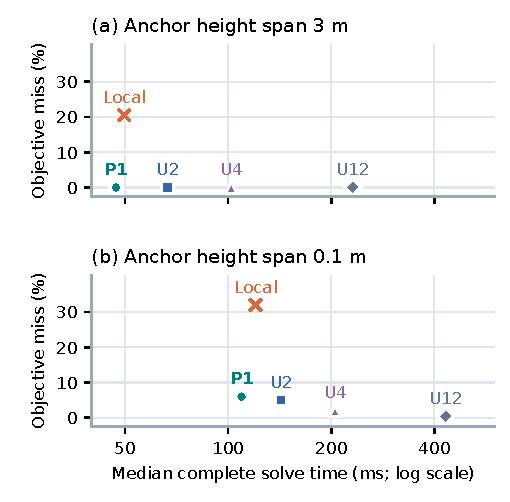
\includegraphics[width=\linewidth]{recovery_bootstrap_figures/candidate_budget_compact.pdf}
 \end{minipage}\hfill
 \begin{minipage}[t]{0.48\textwidth}
  \centering
  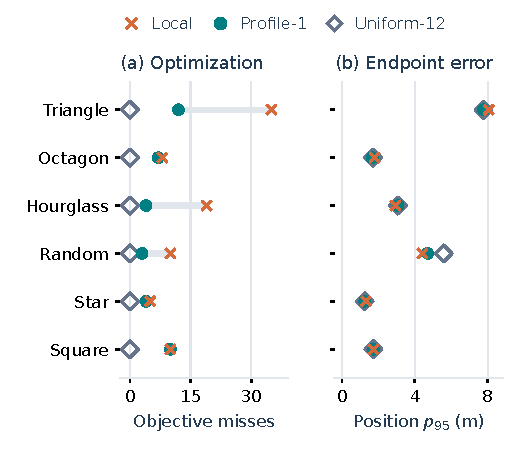
\includegraphics[width=\linewidth]{recovery_bootstrap_figures/real_window_outcomes.pdf}
 \end{minipage}
 \caption{左：两种高度几何下的候选成本与目标miss，时间轴为对数刻度，P1为本文单候选，Uk为均匀k起点。
 右：六条真实日志的目标miss及终点位置p95。青色为本文候选、橙色为Local、菱形为十二起点参考；
 每日志88个相关配置来自11个物理窗口、两个布局及四种等价航向坐标。}
 \label{fig:outcomes}
\end{figure}

在既有30 m、有激励运动中选取3 m与0.1 m两个高度跨度，每种保留原先200个种子。
比较Local、Profile-1、Uniform-2/4/12；同一窗口的测距、平移策略、损失与每次求解限额完全一致。
各策略采用相同的每次求解限额，并报告不同候选数对应的总计算量。
新miss参考五方法找到的最优目标$J_{\rm best}$，阈值
$\max\{10^{-3},10^{-5}|J_{\rm best}|\}$；旧相对十二起点的统计另行保留。
误差p95按全部200例计算，函数评估含两次共同CV和所有航向精化。
耗时来自每种几何前8例、5次交错重复的单进程子集（合计400次），包含投影、求根与曲率，
预热剔除并避开其他数值拟合；本机为i5-12600KF、单BLAS线程。
彩色成本图见图\ref{fig:outcomes}左侧，完整数值表见英文正文。
3 m几何下Profile-1与Uniform-2均无miss，实际中位耗时47.1/66.6 ms，前者少约29.4\%；
0.1 m几何下Profile-1仍有12次miss，双/四/十二起点为10/4/1次；这些方法的位置尾部仍约4 m。
十二起点唯一miss的配置由Profile-1找到更低目标；弱几何下局部法有6次达到评估上限。

\subsection{按日志重汇总真实终点误差}
3168条拟合给出每日志88个相关配置的终点位置误差。
图\ref{fig:outcomes}右侧并列展示目标miss与位置p95，直接比较求解质量与物理精度。
全部528配置的Local/Profile-1/Uniform-12终点RMSE为1.996/1.898/1.926 m，
位置p95为4.241/4.084/4.241 m，统计对象均为窗口终点。
总体位置尾部略有改善；hourglass与random的Profile-1尾部升高，反映不同记录中的位置收益差异。

\section{工作成果与适用范围}
本文完成了从数学结构到初始化算法的闭环：惯性形状与线性干扰消元给出圆上的低成本航向候选，
原始距离精化提供窗口终点状态，不变坐标转换将其交接到共同InEKF。
配对实验显示，在30 m距离、3 m锚点高度跨度下，单候选保持双起点的目标质量，
串行桌面计时子集的中位耗时减少约29.4\%；
真实窗口目标miss由87降至40。多项式不变性、偏置歧义和旋转余项界则给出模型阶数的选择依据。

恢复命题针对精确短窗模型与投影，实际实现采用截断SVD与局部精化。
真实数据来自同日开发日志，离线标定和对齐使用真值，位置结果按相关窗口配置汇总。
完整轨迹在正常测距下实现共同跟踪器接入，断测瞬态仍有较大峰值。
后续重点是独立日期与几何验证、带姿态真值的评估、协方差校准与捕获监督策略。
\end{document}
